\section{Business Model}
\label{sec:BusinessModel}

By analyzing industry trends and identifying opportunities we plan to tailor our business model. This tailored approach aims to not only effectively reach our target audience but also strategically position our offerings amidst competitors. Based on personal experience and the today’s world full of digital content and enormous social media influence, we came to the conclusion that there would not be better way to attract customers than doing so digitally.

Our Coaching Freelancing Platform aims to solve a key problem that the majority of the fitness enthusiasts and health instructors have to face when it comes to online coaching – the absence of communication, the lack of easy-access workouts and direct contact with your trainer and the difficulty of effortlessly finding trainees. Our product provides digital environment where both coaches and trainees benefit from each other. Trainers can create their own profile listing their expertise, awards and pictures, diplomas and certificates, years of experience, area of training, result of previous clients and their feedback. If they already have a greater number of followers, it be extremely easy for them to find clients through the platform. If not, they can promote themselves and rise above other of their colleagues. Additionally, building clients’ workouts won’t be so time consuming and demanding for them as we provide a workout builder with variety of exercise to choose from, set reps and sets and place it in a monthly calendar. Fitness enthusiasts on the other hand will have the easiest way to find someone to help them achieve their health goals. With the ability to filter area of training, years of experience, testimonies, picture-based result, etc., their decision will be trouble-free. Furthermore, we have solved the inability to communicate with your online coach by providing private one-on-one chatting channels between the trainee and the trainer. In those channels, both sides will be provided with statistics of the progress of the customer.

Our business plan includes multiple revenue sources to support. Our primary source of income will come from transactional commissions, where we take a percentage from each coaching transaction made through our platform. Additionally, we will explore revenue streams by letting different sporting brands to promotes their products on our application. Moreover, leveraging a comprehensive database featuring user preferences, gym performance metrics, sleep and dietary habits, as well as body measurements, stands as a pivotal asset.

Having said the wide scope of our web-application, we will have a lot of research and development expenses, programmers’ wages. Additionally, a budget for marketing and advertising fees has to be allocated as well.

We are going to have retail partnership with sports well-known brands who have big influence over the health community. Trainers will have easy access to their accounts through a web-site whereas trainees will be able to download the application from the App Store and Google Play Store.

The key task our team needs to face is the development and deployment of the Coach Freelancing Platform. This includes various stages, including planning, software design and architecture, coding and programming, testing and quality assurance, user interface and experience design, as well as implementation and ongoing maintenance. Additionally, our team will focus on providing continuous support to ensure the platform operates smoothly, addressing any technical issues promptly, and incorporating user feedback to enhance the overall user experience.

Two essential resources critical to building and operating our software are a robust database infrastructure and the intellectual property associated with our application. A well-structured database is fundamental for storing and managing user data, coach profiles, workout routines, and other essential information efficiently. Furthermore, safeguarding the intellectual property rights to our application ensures that our innovative features and functionalities are protected, preventing unauthorized use or replication by competitors.

Two strategic partnerships crucial to our business model are with payment processing platform Stripe and handling transactions efficiently. Integrating with Stripe enables seamless and secure payment transactions on our platform, enhancing user trust and facilitating monetization through commissions. Additionally, partnering with transaction handling services ensures reliable and efficient processing of coaching session payments, reducing friction for users and coaches alike while streamlining our revenue generation process. These partnerships play a vital role in optimizing the financial operations of our Coaching Freelancing Platform and enhancing the overall user experience.

Health and fitness is an industry that is extremely dynamic and develops faster than ever. Therefor agility and adaptability are very important for our business model. By closely monitoring market trends, technological advancements, and user feedback enables us to quickly adapt and improve our platform, adding new features, improving user experience, as well as staying ahead of the competition. Our agile way of working guarantees that Coaching Freelancing Platform adapts to diversifying customer tendencies as well as changing the market situation, thus, ensuring the project’s success in the long-term perspective.

As part of our business analysis we have also prepared a Business Model Canvas, User Personas and Value Proposition Canvases so that we can see a full picture of our business formed by them.

\begin{figure}[H]
    \centering
    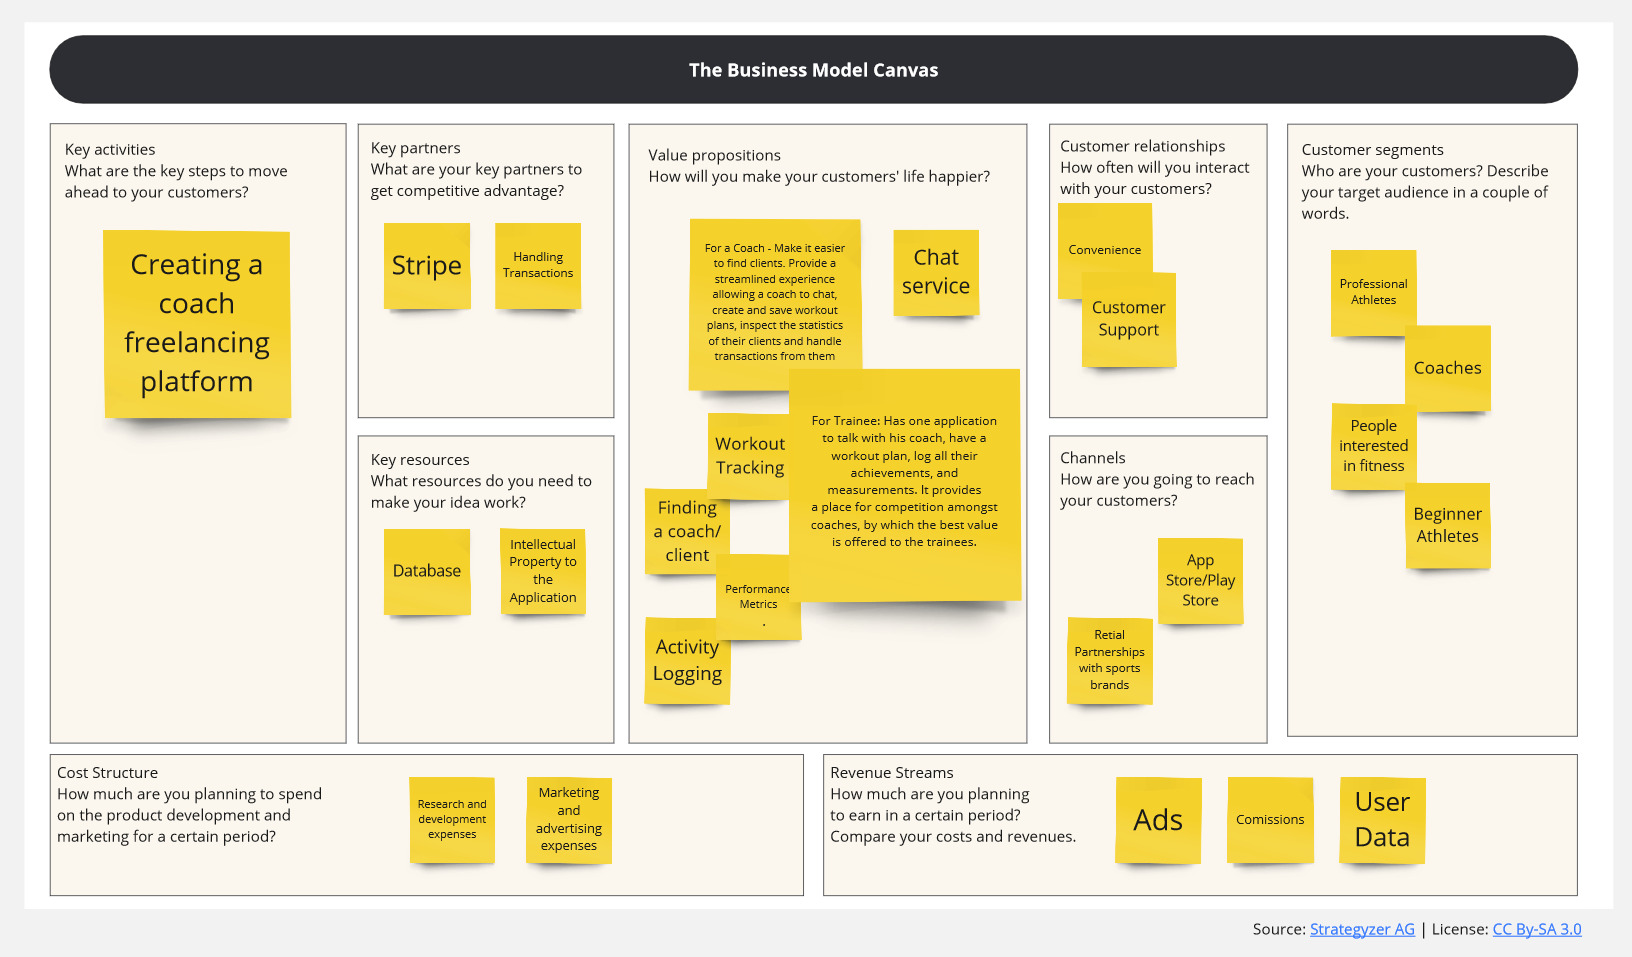
\includegraphics[width=0.8\textwidth]{images/business_model_canvas.jpg}
    \caption{Business Model Canvas}
    \label{fig:businessModel}
\end{figure}

\begin{figure}[H]
    \centering
    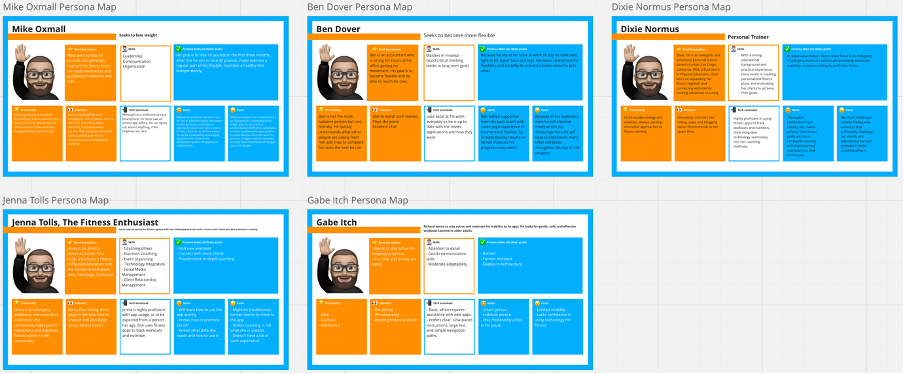
\includegraphics[width=0.8\textwidth]{images/personas.png}
    \caption{Personas}
    \label{fig:personas}
\end{figure}

\begin{figure}[H]
    \centering
    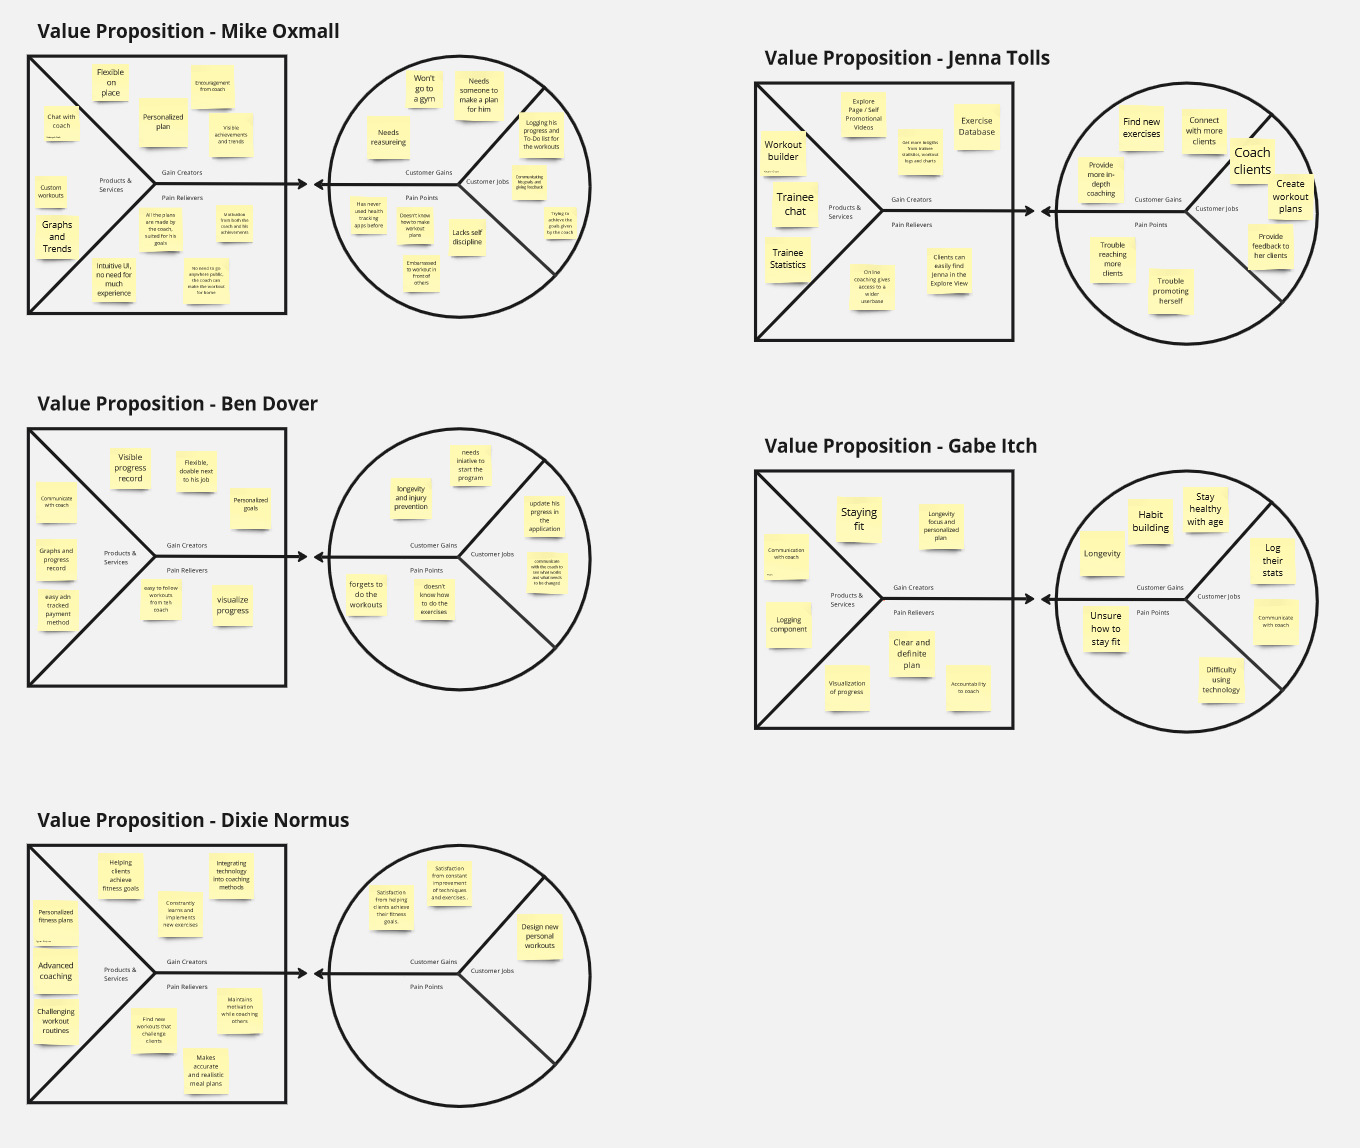
\includegraphics[width=0.8\textwidth]{images/value_proposition_canvas.jpg}
    \caption{Value Proposition Canvases}
    \label{fig:vp}
\end{figure}

\clearpage
